\subsection{Combining FP and PLR Indexing}
\label{sec:combine}

The FP- and PLR-based indexing behaves differently, thereby having different
memory requirements.  
The FP-based indexing requires 7.89-bit per
entry all the time. The PLR-based indexing requires 
51.2-bit per line segment, on average,
and thus its memory efficiency is decided by how many 
$<x_i,y_i>$ pairs are expressed by a line segment. In our setting, 
once each line segment 
can express more than 6.5 $<x_i,y_i>$ pairs, 
PLR outperforms FP, requiring less than 7.89-bit per
entry. Otherwise, using FP-based indexing is more beneficial. 

According to our analysis, the PLR-based indexing begins to outperform FP
when it is used for lower levels in the tree.
This is an expected result.  As a level gets larger in
size, many <$x_i$, $y_i$> pairs are densely sorted over a larger run and thus
can be efficiently expressed by a fewer equations.
We plot the number of bits per mapping entry while varying the run size (the
unit run size is 10GB and the storage capacity is 1TB) in
\FIG{fig:bf-plr-bit}(a).  
\FIG{fig:bf-plr-bit}(b) also shows the number of entries expressed
by a line segment.
%For small runs, the BF-based indexing is better, but as the
%run size grows, the PLR achieves better memory
%efficiency.  

\begin{comment}
%maintains a bitmap
%per entry, the PLR may require less memory as it can express many entries
using a few equations.  However, the memory usage of the PLR highly depends on
which level it is assigned.  \FIG{fig:overall:merged-maps} shows the number of
mapping entries expressed by a single linear equation at $L_i$ (from $L_1$ to
$L_{h-1}$).  As many entries are expressed by a linear equation, the PLR
achieves higher memory efficiency. For the middle levels
($L_1$$\sim$$L_{k-1}$), the PLR coalesces 2$\sim$7.89 entries per
equation.  Let us assume that each component of the linear equation requires
8B, 32B in total.
For the levels $L_1$$\sim$$L_{k-1}$, the PLR requires more memory,
16B$\sim$4.05B per mapping entry, than the typical index table where each entry
is 4B.  However, for the lower levels ($L_k$$\sim$$L_{h-1}$), the PLR
coalesces 8.47$\sim$13.52 entries, becoming more efficient than the
typical index table.  This is an expected result.  As a level gets larger in
size, many <$x_i$, $y_i$> pairs are densely sorted over a larger run and thus
can be efficiently expressed by a fewer equations.  Generally speaking, placing
the PLR in lower levels is beneficial; on the other hand, the BF is preferred
to be placed in middle levels.
\end{comment}

%As will be discussed in \SEC{sec:design}, depending on the implementation of the BF-
%and PLR-based indexing, their memory requirements differ greatly. Moreover, 
%\todo{
Given a specific tree, we can achieve the best memory efficiency
by assigning one (either FP or PLR) 
that requires less memory to each run.
However, depending on how the LSM-tree is organized, the size of levels and runs changes,
which affects the assignment of the approximation algorithm.  
We discuss this issue in detail in \SEC{sec:design:tree},
while exploring various organizations of the LSM-tree.


\begin{comment}
The BF- and PLR-based indexing behaves differently, thereby having different
memory requirements.  Compared to the BF-based indexing that maintains a bitmap
per entry, the PLR may require less memory as it can express many entries
using a few equations.  However, the memory usage of the PLR highly depends on
which level it is assigned.  \FIG{fig:overall:merged-maps} shows the number of
mapping entries expressed by a single linear equation at $L_i$ (from $L_1$ to
$L_{h-1}$).  As many entries are expressed by a linear equation, the PLR
achieves higher memory efficiency. For the middle levels
($L_1$$\sim$$L_{k-1}$), the PLR coalesces 2$\sim$7.89 entries per
equation.  Let us assume that each component of the linear equation requires
8B, 32B in total.
For the levels $L_1$$\sim$$L_{k-1}$, the PLR requires more memory,
16B$\sim$4.05B per mapping entry, than the typical index table where each entry
is 4B.  However, for the lower levels ($L_k$$\sim$$L_{h-1}$), the PLR
coalesces 8.47$\sim$13.52 entries, becoming more efficient than the
typical index table.  This is an expected result.  As a level gets larger in
size, many <$x_i$, $y_i$> pairs are densely sorted over a larger run and thus
can be efficiently expressed by a fewer equations.  Generally speaking, placing
the PLR in lower levels is beneficial; on the other hand, the BF is preferred
to be placed in middle levels.

As will be discussed in \SEC{sec:design}, depending on the implementation of the BF-
and PLR-based indexing, their memory requirements differ greatly. Moreover, 
depending on how the LSM-tree is organized, the size of levels and runs changes,
which affects the assignment of the approximation algorithm.  
We discuss this issue in detail in \SEC{sec:design:tree},
while exploring various organizations of the LSM-tree.
\end{comment}


\begin{comment}
In the middle levels ($L_1$$\sim$$L_{k-1}$), PLR-indexing does not coalesce
mapping entries enough to overcome its memory requirement.  As the runs in the
middle levels have fewer mapping entries, they have sparsely sorted mapping
pairs that make the memory efficiency of PLR-indexing worse.  Thus, we place
BF-indexing in the middle levels since BF-indexing always has the same memory
usage under the same FPR.  As the better memory-efficient approximate
algorithms are different by level, we assign the proper indexing algorithms to
level before running.  But, the memory-efficient setup for approximate
techniques may harm I/O performance and the total memory requirements of
\OURS{}.  To figure out the appropriate setup, we explore various \OURS{}
parameters by considering \ours{}'s I/O performance and memory usage in
\SEC{sec:design:tree}.
\end{comment}


\begin{comment}
\begin{figure}[t]
\centering
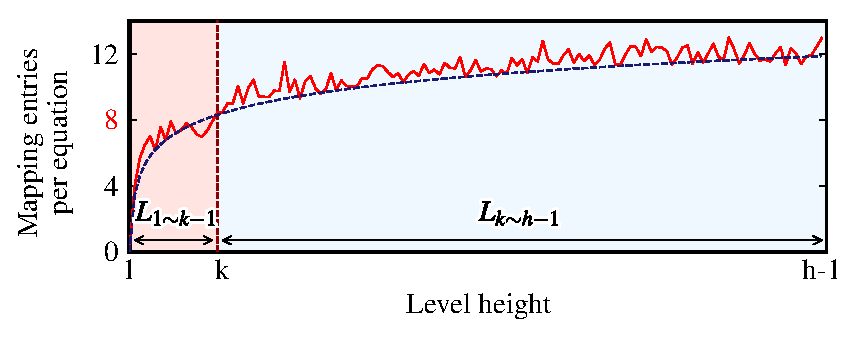
\includegraphics[width=0.4\textwidth]{figs/figs-final/revised/level-PLR.eps}
\vspace{-10pt}
%\caption{\fixme{The number of mapping entries in a function of PLR}}
\caption{The number of mapping entries per PLR equation}
\vspace{-10pt}
\label{fig:overall:merged-maps}
\end{figure}
\end{comment}


\begin{comment}
\todo{
The BF- and PLR-based indexing behaves differently, thereby having different
characteristics, in terms of indexing building cost, memory
efficiency, and lookup latency.  Compared to the BF-based indexing that 
builds tables by invoking a hash function supported by CPU instructions,
rebuilding PLR models takes longer as it requires many arithmetic operations.
Conversely, the PLR models exhibit high compression ratio as the size of a run gets larger.
This is because mapping pairs are likely to be densely sorted in the run,
which enables us to express many mapping pairs using fewer linear functions.
On the other hand, the BF-based indexing suffers from long lookup latency over a large run
because it perform search operations (\ie~binary search and scanning) over a larger run.
Those observations lead us to use the BF-based indexing on middle level where
runs are relatively small in size and compaction (\ie~model rebuilding) is
frequently triggered.  On the other hand, the PLR-based indexing is suitable
for lower levels that have larger runs and where compaction occasionally
happens.}  \todo{In \SEC{todo}, we explain the best cutting of the levels for BF
and PLR; 최적의 장소를 찾는 것은 시뮬레이션으로 할 수 있기 때문에 쉬움.
대신 최적의 메모리와 성능을 찾을 수 있도록 tree를 organization하는것은 생각이 필요함... 
이 부분이 강조 되어야할 듯..}
\begin{figure}[t]
\centering
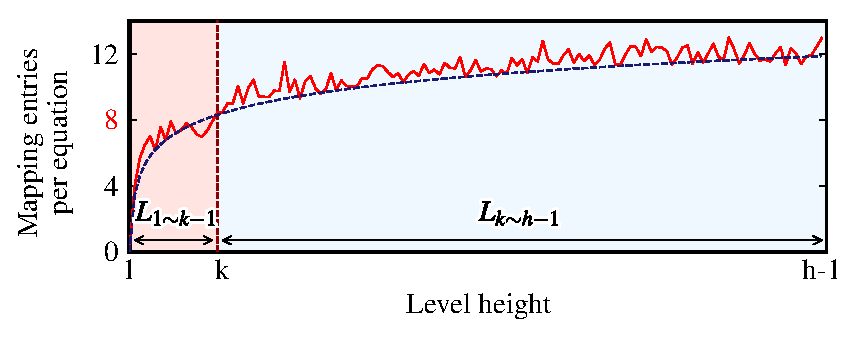
\includegraphics[width=0.345\textwidth]{figs/figs-final/revised/level-PLR.eps}
\caption{\fixme{The number of mapping entries in a function of PLR}}
\label{fig:overall:merged-maps}
\end{figure}

\JS{윗 문단 대신 적으면 좋을듯. 
Because the each function in PLR-indexing manages many mapping entries,
PLR-based indexing has usually less memory requirement than BF-indexing.
However, the memory usage of PLR-indexing highly depends on where runs are
placed.  \FIG{fig:overall:merged-maps} shows the number of coalesced mapping
entries in each PLR function on different levels (\ie~$L_1$$\sim$$L_{h-1}$).
In the middle levels ($L_1$$\sim$$L_{k-1}$), PLR-indexing does not coalesce
mapping entries enough to overcome its memory requirement.  As the runs in the
middle levels have fewer mapping entries, they have sparsely sorted mapping
pairs that make the memory efficiency of PLR-indexing worse.  Thus, we place
BF-indexing in the middle levels since BF-indexing always has the same memory
usage under the same FPR.  As the better memory-efficient approximate
algorithms are different by level, we assign the proper indexing algorithms to
level before running.  But, the memory-efficient setup for approximate
techniques may harm I/O performance and the total memory requirements of
\OURS{}.  To figure out the appropriate setup, we explore various \OURS{}
parameters by considering \ours{}'s I/O performance and memory usage in
\SEC{sec:design:tree}.
}
\end{comment}

%\subsection{Impact of Tree organization on Memory and WAF}
%\subsection{Approximate Indexing using BF and PLR}



